\begin{frame}{Inne humorystyczne języki}
    \begin{columns}
        \begin{column}{.6\hsize}
            {\large Folders}
            \begin{itemize}
                \myitem Daniel Temkin, 2015
                \myitem Kodem źródłowym jest struktura folderów
            \end{itemize}
        \end{column}
        \begin{column}{.45\hsize}
            \begin{figure}
                {\hspace{0cm}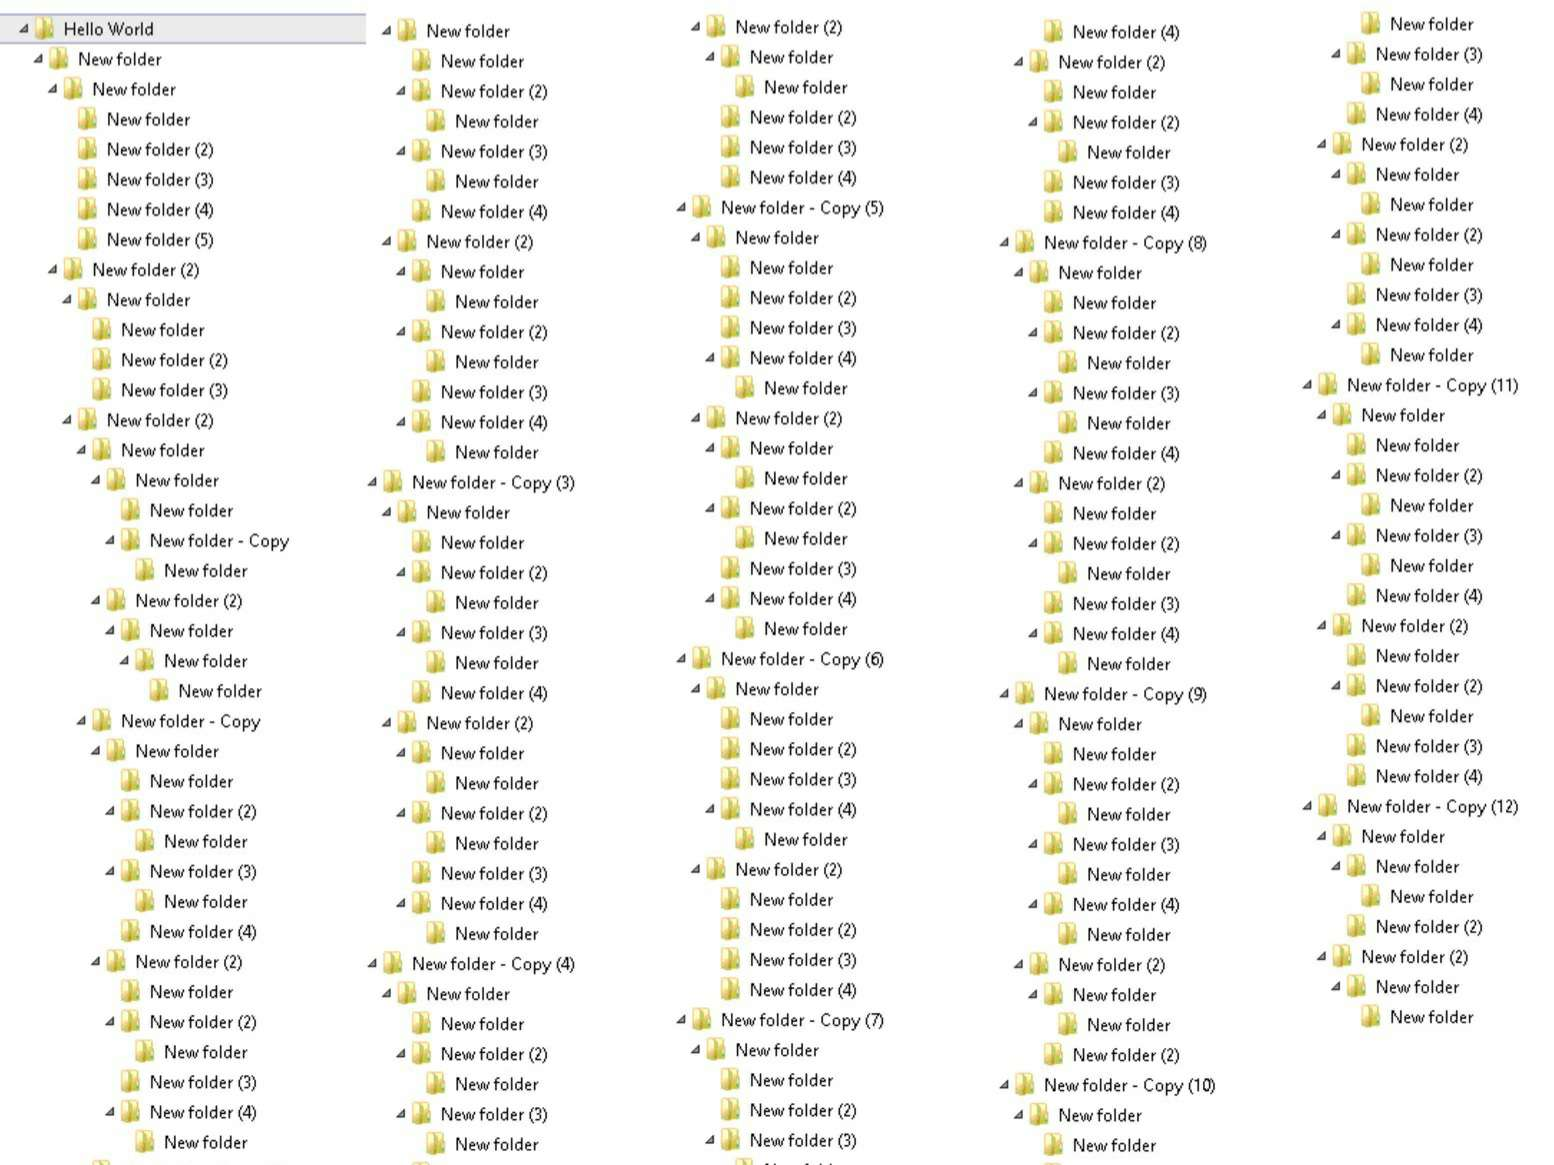
\includegraphics[height=2.5cm]{figures/folders.jpg}}
                \caption*{\scriptsize Folders, ,,Hello World!''{\color{blue} \hyperlink{frame:przypisy}{(8)}}}
            \end{figure}
        \end{column}
    \end{columns}

    \begin{columns}
        \begin{column}{.6\hsize}
            {\large Whitespace}
            \begin{itemize}
                \myitem Edwin Brady \& Chris Morris, 2003
                \myitem Jedynymi rozpoznawanymi znakami są spacja, tab i nowa linia
            \end{itemize}
        \end{column}
        \begin{column}{.45\hsize}
            \begin{figure}
                {\hspace{0cm}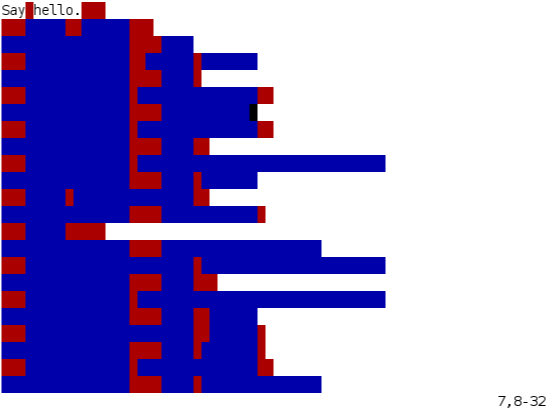
\includegraphics[height=2.5cm]{figures/whitespace.png}}
                \caption*{\scriptsize Whitespace, ,,Hello''{\color{blue} \hyperlink{frame:przypisy}{(9)}}}
            \end{figure}
        \end{column}
    \end{columns}

    % \begin{columns}
    %     \begin{column}{.65\hsize}
    %     \end{column}
    % \end{columns}
\end{frame}